	\chapter{Обилие {\it Macoma balthica}}
	\section{Белое море}
Данные по численности маком в Кандалакшском заливе Белого моря получены для $10$ участков (рис.~\ref{ris:N_area_White}), всего $140$ пространственно-временных точек оценки.
	\begin{figure}[p]
	\begin{center}
		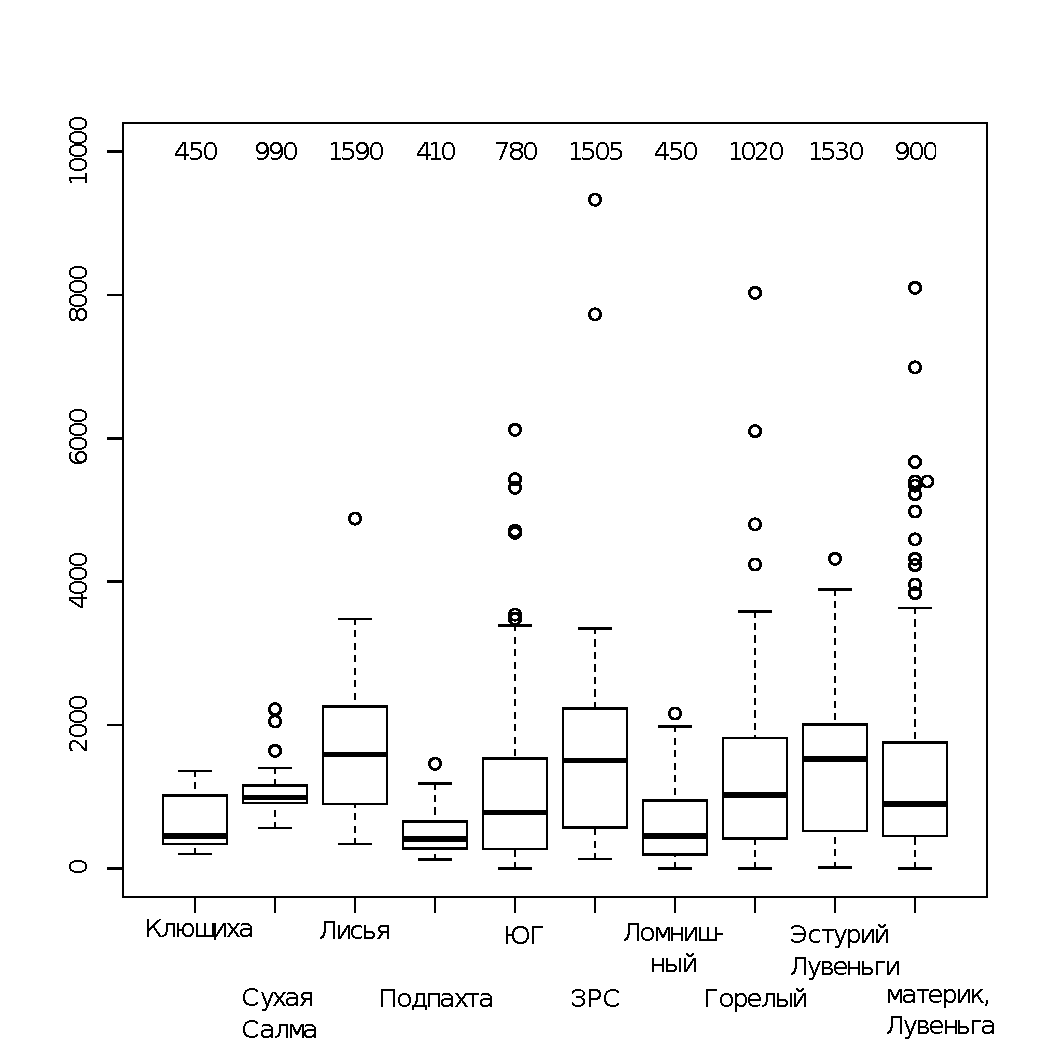
\includegraphics[height=0.5\textheight]{../All_N/N2_area_White1.pdf}
	\end{center}
	\caption{Варьирование средней численности {\it Macoma balthica} на различных участках Кандалакшского залива Белого моря}
	{\footnotesize Примечание: По оси абсцисс --- численность {\it M.~balthica}, ~экз./м$^2$.

	На графике: жирная горизонтальная линия --- медиана, границы <<ящика>> --- 1 и 3 квартили, <<усы>> --- $1,5$ интерквартильного расстояния, точки - значения выпадающие за $1,5$ интерквартильных расстояния

Числа в верхней части графика --- медианное значение численности {\it M.~balthica}, экз./м$^2$}
	\label{ris:N_area_White}
	\end{figure}
Средняя численность особей {\it M.~balthica} была представлена в диапазоне от $10$ (о.~Горелый) до $8500$~экз./м$^2$ (Западная Ряшкова салма) (табл. \ref{tab:mean_NB_White}, Приложение~\ref{app:NB_table}).

%
Однако экстремально высокие численности --- более $2800$~экз./м$^2$ --- встречаются единично, всего $8$ наблюдений из $140$ (рис. \ref{ris:Nmean_hist}).
%
	\begin{figure}[p]
		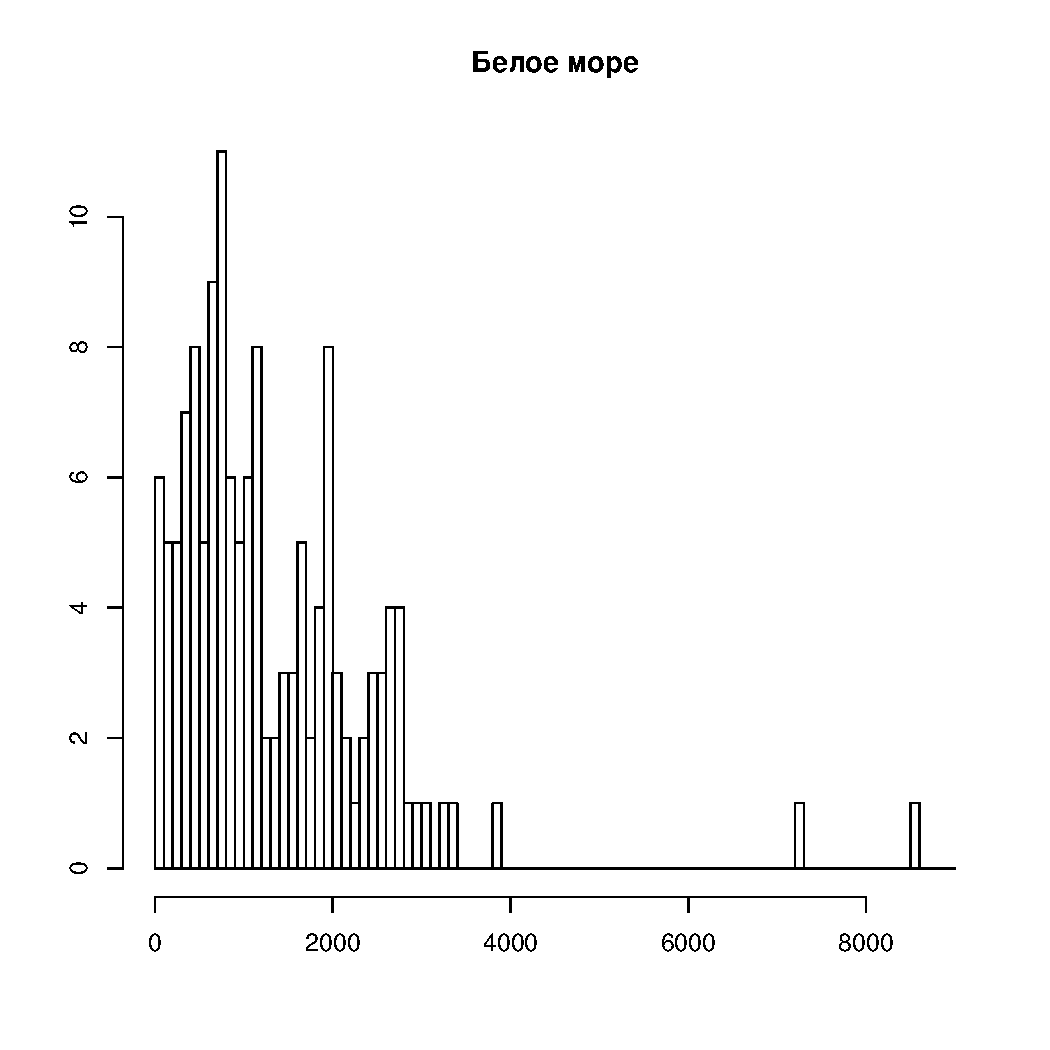
\includegraphics[height=.3\textheight]{../All_N/Nmean_hist_White1.pdf}
		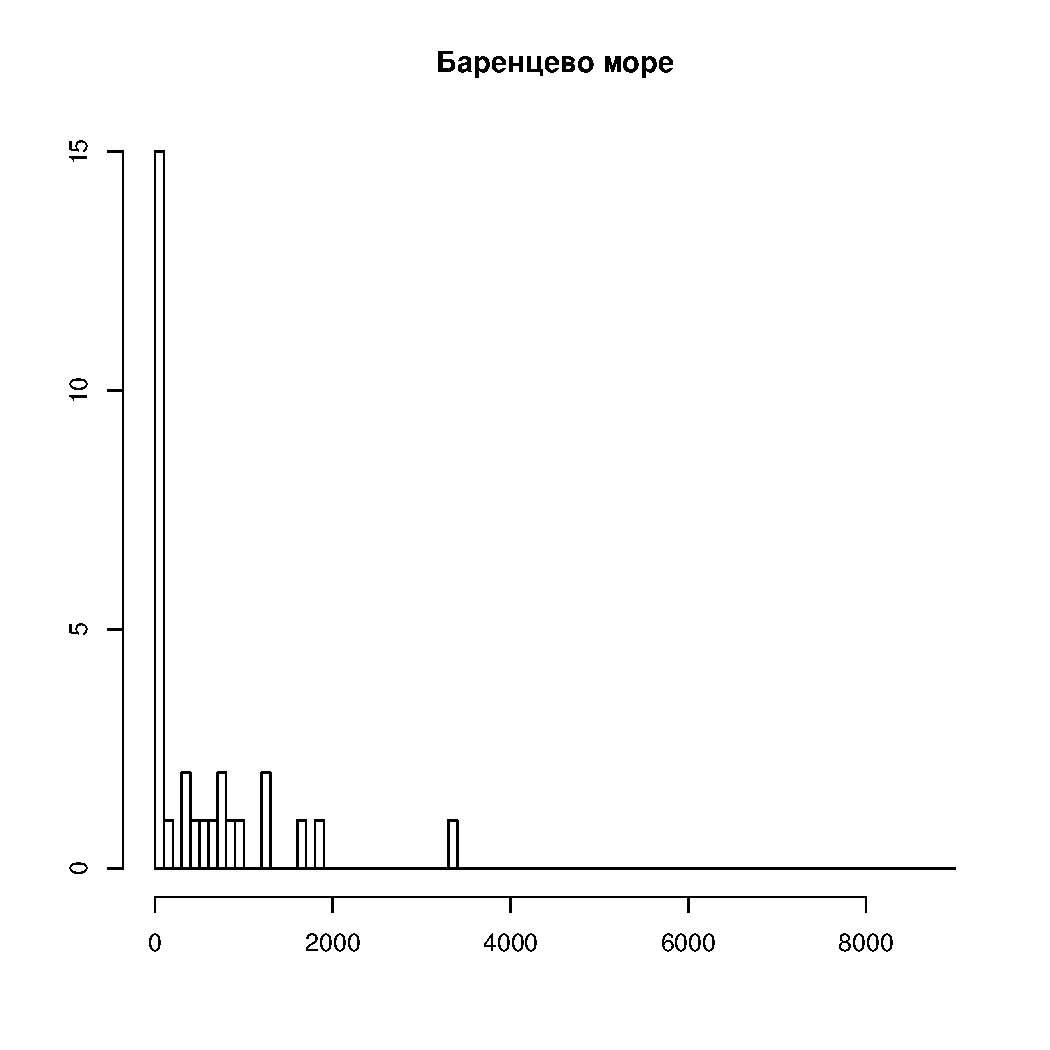
\includegraphics[height=.3\textheight]{../All_N/Nmean_hist_Barents1.pdf}
	\caption{Частота встречаемости поселений с различным обилием {\it Macoma balthica}}
	{\footnotesize Примечание: по оси $X$ --- средняя численность {\it Macoma balthica}, экз./м$^2$ (шаг --- $100$~экз./м$^2$), по оси $Y$ 	--- частота встречаемости}
	\label{ris:Nmean_hist}
	\end{figure}
%
Наиболее часто встречаются поселения со средней численностью $700-800$~экз./м$^2$.
Отдельные районы Кандалакшского залива Белого моря не отличались по средней численности маком ($Kruskal-Wallis\ \chi^2 = 5,6$, $p = 0,2$). 
При сравнении средних обилий маком на разных участках в пределах одного горизонта не показало достоверных отличий (табл.~\ref{tab:Nmean_Kruskal_mareography_White}).
%
	\begin{table}[p]
            \caption{Сравнение средней численности {\it M.~balthica} в пределах одного мареографического уровня в Белом море}
            \label{tab:Nmean_Kruskal_mareography_White}
        \begin{center}
            \begin{tabular}{|*{4}{p{0.2\textwidth}|}} \hline
                ма\-ре\-ографи\-ческий уровень & $Kruskal-Wallis\ \chi^2$ & $df$ & $p$ \\
                \hline
                СГЛ & $2,7$ & $5$ & $0,7$ \\
                \hline
                НГЛ & $5,8$ & $4$ & $0,2$ \\
                \hline
                ноль глубин & $0,16$ & $1$ & $0,7$ \\
                \hline
                ВСЛ & $1$ & $1$ & $0,3$ \\
                \hline
            \end{tabular}
        \end{center}

	{\footnotesize Примечания: градации мареографического уровня: ВГЛ --- верхний горизонт литорали, СГЛ --- средний горизонт литорали, НГЛ --- нижний горизонт литорали, ВСЛ --- верхняя сублитораль}
	\end{table}
%
    Сравнение средних численностей на разных горизонтах в пределах одного участка показало различные результаты (табл.~\ref{tab:N2_area_mareography_Kruskal_White}). 
%
	\begin{table}[p]
	\caption{Сравнение численности {\it M.~balthica} в поселениях на разном мареографическом уровне в Белом море}
	\label{tab:N2_area_mareography_Kruskal_White}
        \begin{center}
        \begin{tabular}{|p{0.25\textwidth}|*{4}{p{0.15\textwidth}|}} \hline
    участок & $Kruskal-Wallis\ \chi^2$ & $df$ & $p$ & \\
	\hline
    Клющиха & $19,7$ & $2$ & $5,2 \times 10^{-05}$ & ***\\
    \hline
    Клющиха (только литораль) & $1,1$ & $1$ & $0,31$ & \\
    \hline
    Сухая & $0,0057$ & $1$ & $0,94$ & \\
    \hline
    Лисья & $17,5$ & $2$ & $0,00016$ & ***\\
    \hline
    Лисья (только литораль) & $11,06$ & $1$ & $0,00088$ & ***\\
    \hline
    Подпахта  & $2,3$ & $1$ & $0,13$ & \\
    \hline
    Горелый & $10,2$ & $3$ & $0,01658$ & ** \\
    \hline
    материк, Лувеньга & $2,4$ & $3$ & $0,50$ &  \\
    \hline
	\end{tabular}
        \end{center}

    {\footnotesize Примечание: достоверность различий *** --- $p<0,001$; ** --- $p<0,05$; * --- $p<0,1$.}
	\end{table}
%
Для участков в Сухой салме, проливе Подпахта, материковой литорали в Лувеньге варьирование численности между пробами перекрывало варьирование между горизонтами литорали.
При этом для участков в бухтах Клющиха и Лисья и на о.~Горелом Лувеньгских шхер  было показано достоверное влияние мареографического уровня на обилие маком. 
Интересно отметить, что в бухте Клющиха численность маком на нижнем и среднем горизонтах литорали не отличается ($403$~($7$\%)\footnote{здесь и далее в скобках указана точность учета d, \%}~экз./м$^2$), но в сублиторали она значительно выше ($1136$~($5$\%)~экз./м$^2$).
В бухте Лисья ситуация отличается, обилие маком на нижнем горизонте достоверно выше ($2832$~($10$\%)~экз./м$^2$), чем в среднем и в сублиторали ($1346$~($16$\%) и $1006$~($16$\%)~экз./м$^2$, соответственно). 

Данные по биомассе {\it M.~balthica} были получены для $10$ участков, всего $133$ про\-стран\-ствен\-но-вре\-мен\-ных среза. 
Размах варьирования средней биомассы был от $1,1$~($25$\%)~г/м$^2$ (б.~Клющиха, $2006$~год) до $177,9$~($9$\%)~г/м$^2$ (о.~Горелый, $2004$~год) (табл. \ref{tab:mean_NB_White}, Приложение~\ref{app:NB_table}).

Средняя биомасса маком на участках в губе Чупа по нашим данным была ниже, чем в остальных двух районах ($Kruskal-Wallis~\chi^2 = 12,5$; $p = 0,002$) (рис.~\ref{ris:B_region_White}).
	\begin{figure}[p]
	\begin{center}	
		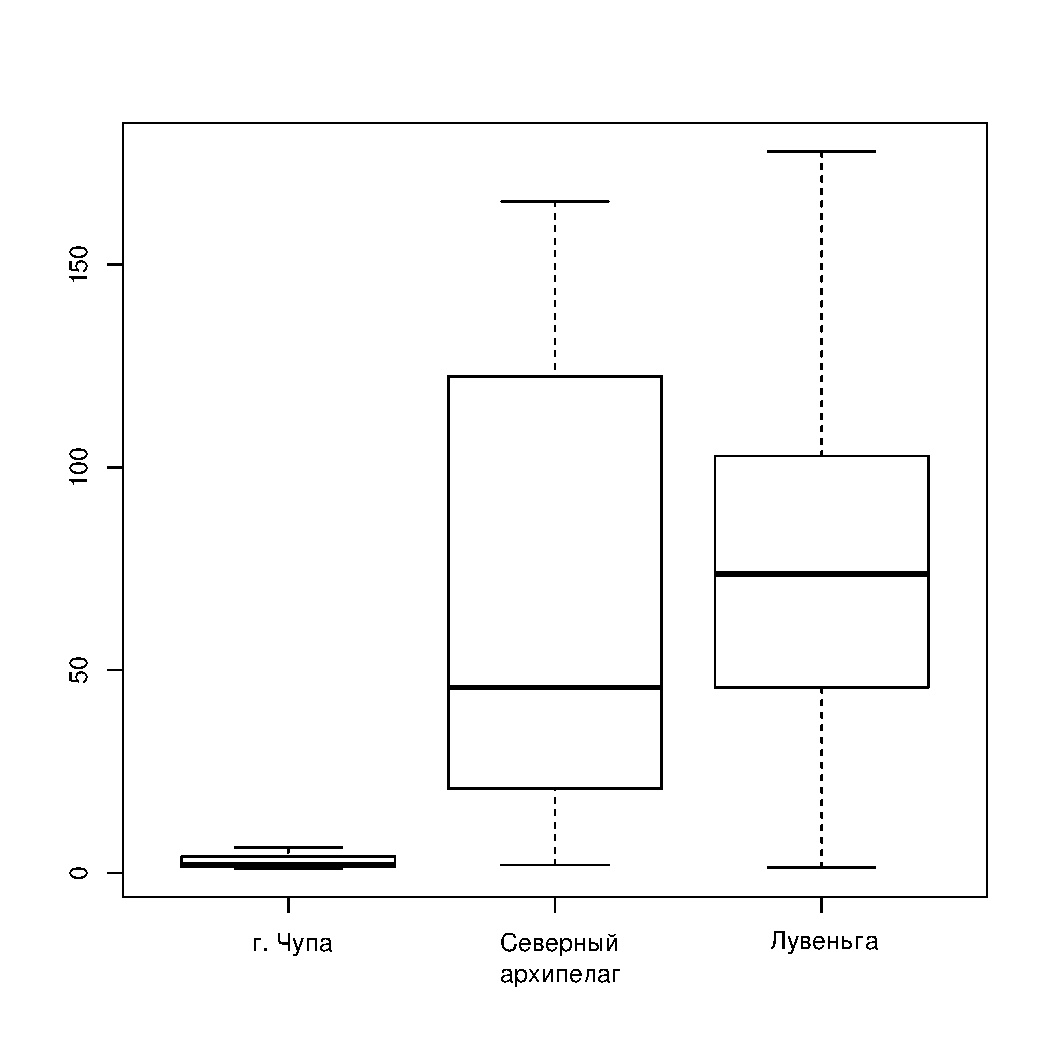
\includegraphics[height=0.5\textheight]{../All_B/Bmean_region_White1.pdf}
	\end{center}
	\caption{Варьирование средней биомассы {\it Macoma balthica} в разных районах Кандалакшского залива Белого моря}
	{\footnotesize Примечание: По оси абсцисс --- биомасса {\it M.~balthica},~г/м$^2$.

	На графике: жирная горизонтальная линия --- медиана, границы <<ящика>> --- 1 и 3 квартили, <<усы>> --- $1,5$ интерквартильного расстояния, точки - значения выпадающие за $1,5$ интерквартильных расстояния}
	\label{ris:B_region_White}
	\end{figure}

\afterpage{\clearpage}

%%%%%%%%%%%%%%%%%%%%%%%%%%%%%%%%%%%%%%%%%%%%%%%%%%%%%%%%
	\section{Баренцево море}

В Баренцевом море данные по обилию маком были получены для $12$ участков Мурманского побережья (рис~\ref{ris:N_area_Barents}).
	\begin{figure}[p]
	\begin{center}
		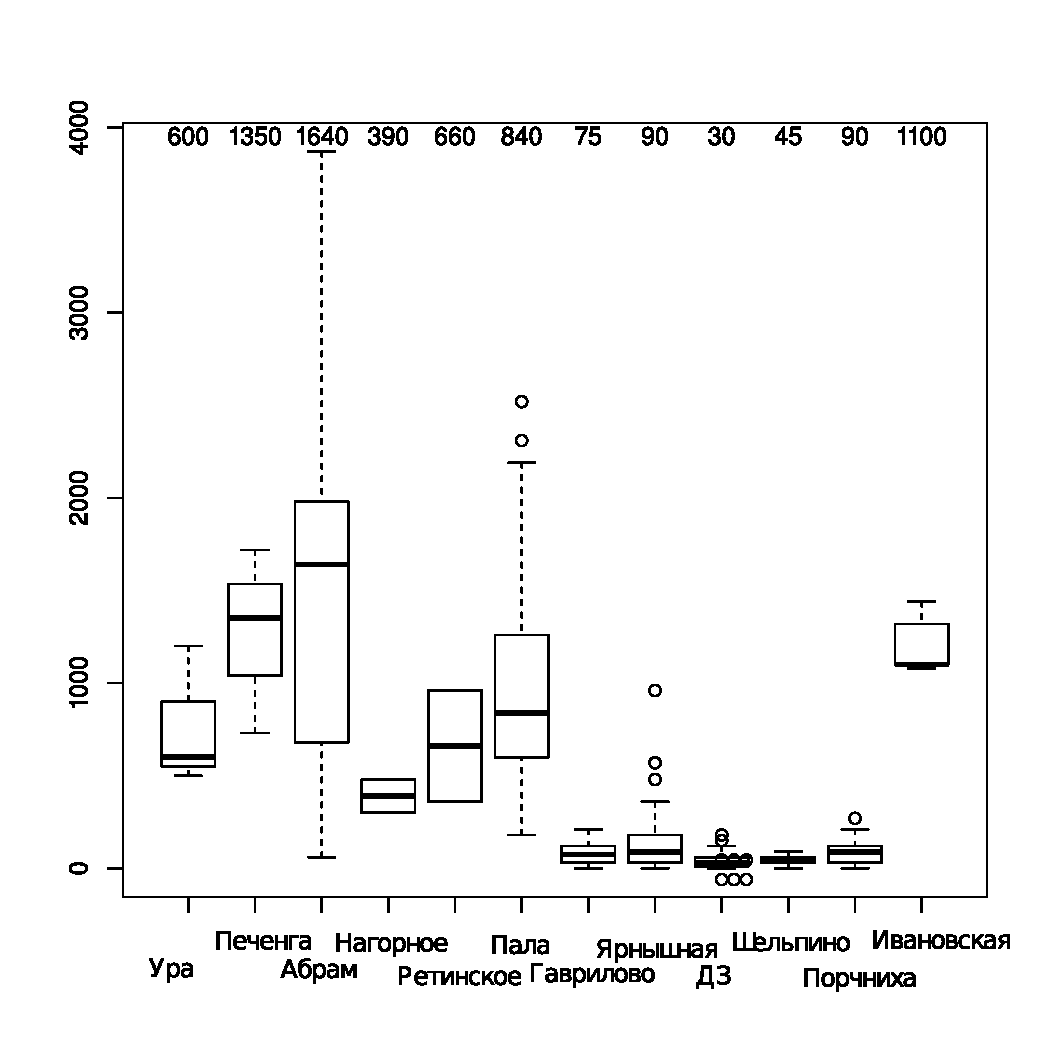
\includegraphics[height=0.5\textheight]{../All_N/N2_area_Barents1.pdf}
	\end{center}
	\caption{Варьирование средней численности {\it Macoma balthica} на различных участках Мурманского побережья Баренцева моря}
	{\footnotesize Примечание: По оси абсцисс --- численность {\it M.~balthica}, ~экз./м$^2$.

	На графике: жирная горизонтальная линия --- медиана, границы <<ящика>> --- 1 и 3 квартили, <<усы>> --- $1,5$ интерквартильного расстояния, точки - значения выпадающие за $1,5$ интерквартильных расстояния}
	\label{ris:N_area_Barents}
	\end{figure}
Минимальная средняя численность составляла $30$~экз./м$^2$ (г.~Дальне-Зеленецкая), что сравнимо с показателями для Белого моря. 
Максимальная средняя численность была значительно меньше, чем беломорская --- $3350$~экз./м$^2$ (Абрам-мыс) (табл.~\ref{tab:mean_NB_Barents}, Приложение~\ref{app:NB_table}). 
Среди исследованных, наиболее часто встречались поселения со средним обилием менее $100$~экз./м$^2$ (рис.~\ref{ris:Nmean_hist}).

Для Мурманского побережья Баренцева моря показаны различия между отдельными районами: Западным, Восточным Мурманом и Кольским заливом (\cite{Guryanova_Ushakov_1929, Guryanova_et_al_1930}). 
Это подтверждается нашими данными (рис.~\ref{ris:N_region_Barents}) по размаху варьирования среднего обилия в пределах районов ($Kruskal-Wallis\ \chi^2 = 17,6$, $p = 0,00015$).
%
	\begin{figure}[p]
	\begin{center}
		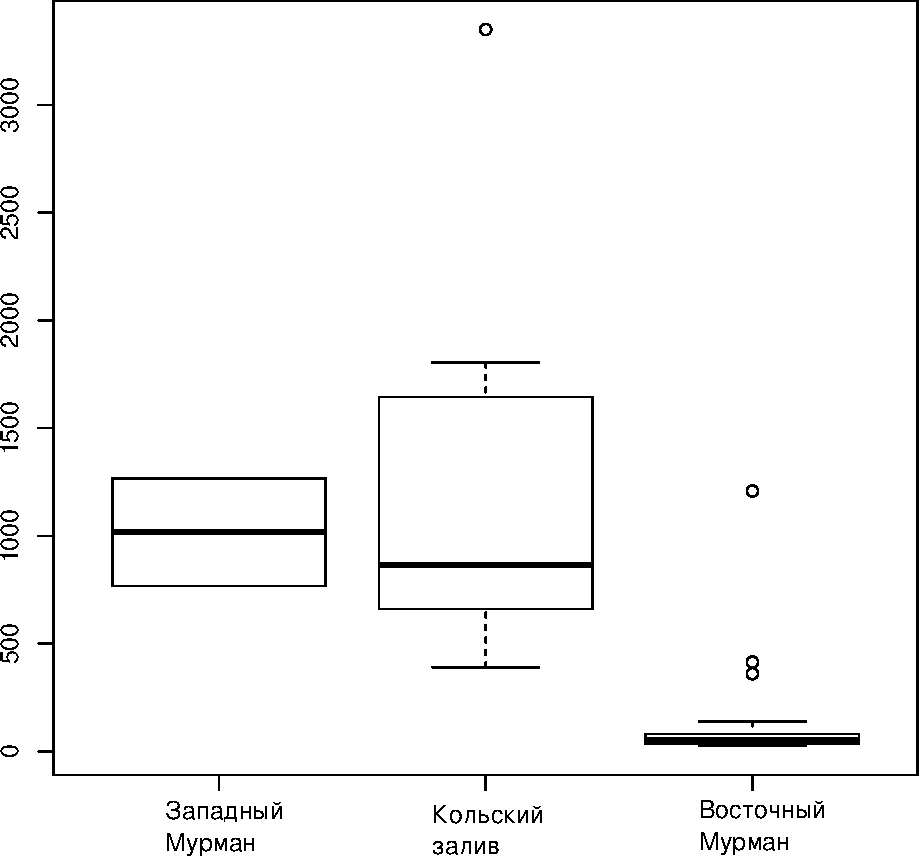
\includegraphics[height=0.5\textheight]{../All_N/Nmean_region_Barents1.pdf}
	\end{center}
	\caption{Варьирование средней численности {\it Macoma balthica} в разных районах Мурманского побережья Баренцева моря}
	{\footnotesize Примечание: По оси абсцисс --- численность {\it M.~balthica}, ~экз./м$^2$.

	На графике: жирная горизонтальная линия --- медиана, границы ''ящика'' --- 1 и 3 квартили, ''усы'' --- $1,5$ интерквартильного расстояния, точки - значения выпадающие за $1,5$ интерквартильных расстояния

Числа в верхней части графика --- медианное значение численности {\it M.~balthica}, экз./м$^2$}
	\label{ris:N_region_Barents}
	\end{figure}
%
На литорали Восточного Мурмана численность {\it M.~balthica} в основном не превышала $100$~экз./м$^2$. 
Единственное исключение ---\ литораль губы Ярнышная, где численность маком достигала $410$~($12$\%)~экз./м$^2$. 
Между тем, на единственном участке, где были учеты в сублиторали, в губе Ивановской, численность на порядок выше, чем ее значения на литорали Восточного Мурмана, и составляет $1200$~экз./м$^2$. 
В Кольском заливе минимальные значения обилия были отмечены на литорали в районе Северного Нагорного ($390$~($23$\%)~экз./м$^2$). 
%Данный участок находится ближе всего к куту Кольского залива из всех исследованных, и характеризуется сильным распресненных. 
Максимальных значений численности как для региона, так и для всей исследованной части Мурманского побережья, достигали поселения маком на участке в районе Абрам-мыса ($3350$~($16$\%)~экз./м$^2$). 
На Западном Мурмане обилие флуктуировало вокруг значения $1000$~экз./м$^2$.  

При сравнении численности маком на различных мареографических уровнях различия между горизонтами литорали были показаны для губ Гаврилово и Ярнышная (табл.~\ref{tab:N2_area_mareography_Kruskal_Barents}).
В Гаврилово средняя численность {\it M.~balthica} в среднем горизонте литорали превышала аналогичные значения для нижнего горизонта на порядок ($138$~($15$\%) и $24$~($47$\%)~экз./м$^2$, соответственно).
В губе Ярнышная численность маком в верхнем и нижнем горизонтах не различалась ($414$~($12$\%) и $360$~($43$\%)~экз./м$^2$, соответственно), в то время как в среднем горизонте литорали она была значительно ниже ($70$~($14$\%)~экз./м$^2$).  
%
	\begin{table}[p]
	\caption{Сравнение численности {\it Macoma balthica} в поселениях на разном мареографическом уровне в Баренцевом море}
	\label{tab:N2_area_mareography_Kruskal_Barents}
    \begin{center}
        \begin{tabular}{|p{0.25\textwidth}|*{4}{p{0.15\textwidth}|}} \hline
    участок & $Kruskal-Wallis\ \chi^2$ & $df$ & $p$ & \\
    \hline
    Абрам-мыс &  $1,5$ & $1$ & $0,224$ & \\
    \hline
    Пала-губа & $0,4$ & $1$ & $0,54$ & \\
    \hline
    Гаврилово & $6,9$ & $1$ & $0,0084$ & *** \\
    \hline
    Ярнышная & $19,4$ &  $2$ &  $6,09 \times 10^{-5}$ & *** \\
    \hline
    Дальне-Зеленецкая & $1,6$ & $2$ & $0,45$ & \\
    \hline
    Шельпино & $0,7$ & $1$ & $0,39$ & \\
    \hline
	\end{tabular}
    \end{center}

    {\footnotesize Примечание: достоверность различий *** --- $p<0,001$; ** --- $p<0,05$; * --- $p<0,1$.}
	\end{table}
%

Для Баренцева моря биомасса была получена только для $2$ участков в Кольском заливе и $6$ участков на Восточном Мурмане, всего $17$ про\-стран\-ствен\-но-вре\-мен\-ных срезов. 
Средняя биомасса маком в Баренцевом море варьировала от $13,0~(53\%)$~г/м$^2$ (Гаврилово) до $216,5~(25\%)$~г/м$^2$ (Абрам-мыс) (табл.~\ref{tab:mean_NB_Barents}, Приложение~\ref{app:NB_table}).

Средняя биомасса в Кольском заливе была выше, чем на Восточном Мурмане ($Kruskal-Wallis~\chi^2 = 6,8$; $p = 0,009$) (рис.~\ref{ris:B_region_Barents}).
	\begin{figure}[p]
	\begin{center}	
		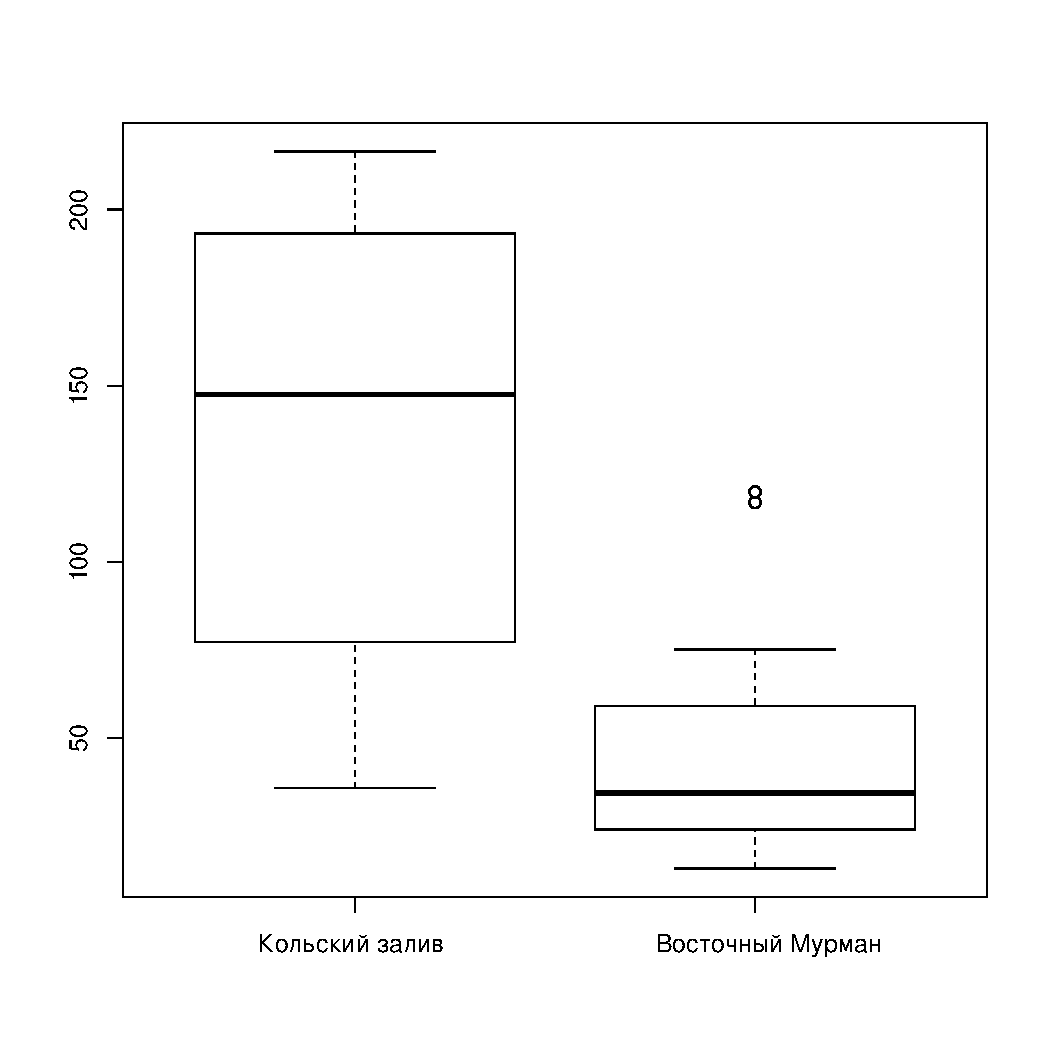
\includegraphics[height=0.5\textheight]{../All_B/Bmean_region_Barents1.pdf}
	\end{center}
	\caption{Варьирование средней биомассы {\it Macoma balthica} в разных районах Баренцева моря}
	{\footnotesize Примечание: По оси абсцисс --- биомасса {\it M.~balthica},~г/м$^2$.

	На графике: жирная горизонтальная линия --- медиана, границы <<ящика>> --- 1 и 3 квартили, <<усы>> --- $1,5$ интерквартильного расстояния, точки - значения выпадающие за $1,5$ интерквартильных расстояния}
	\label{ris:B_region_Barents}
	\end{figure}


\afterpage{\clearpage}

%%%%%%%%%%%%%%%%%%%%%%%%%%%%%%%%%%%%%%%%%%%%%%%%%%%%%%%%%%%%%%%%%%%%%%%
    \section{Влияние состава грунта на численность {\it Macoma balthica}}
Нет сомнений, что основной параметр, определяющий обилие маком~---\ это доступные пищевые   ресурсы.   
Косвенным   показателем   наличия   пищевых   ресурсов   служит гранулометрический состав грунта и общее содержание органических веществ. 

Поскольку для Белого моря были доступны многолетние ряды, то для анализа связи обилия маком с гранулометрическим составом грунта мы использовали средние многолетние и максимальные значения численности маком на участках. 
Для литорали на о.~Горелом мы использовали данные по отдельным горизонтам литорали.
Достоверная положительная корреляция обилия маком была обнаружена с гравием и крупным песком (табл.~\ref{tab:grunt_N_correlation_White}).
	\begin{table}[p]
	\begin{center}
		\caption{Сравнение средней ($N_{mean}$) и максимальной ($N_{max}$) численности {\it Macoma balthica} на литорали с различным гранулометрическим составом грунта в Белом море}
	\label{tab:grunt_N_correlation_White}
	\begin{tabularx}{\textwidth}{|l|XXl|XXl|}
	\hline
	& \multicolumn{3}{c|}{$N_{mean}$} & \multicolumn{3}{c|}{$N_{max}$}\\ \hline
           & $R_s$ & $p-value$ &    & $R_s$ & $p-value$ &     \\ \hline
	$> 10$~мм   & -0,25     & 0,56    &    & -0,11    & 0,80   &     \\ \hline
	$5 - 1$~мм  & 0,74      & 0,05    & *  & 0,81     & 0,02   & **  \\ \hline
	$1 - 0,5$мм  & 0,83      & 0,02    & ** & 0,95     & 0,00   & *** \\ \hline
	$0,5 - 0,25$~мм & 0,64      & 0,10    &    & 0,55     & 0,17   &     \\ \hline
	$0,25 - 0,1$~мм  & -0,62     & 0,11    &    & -0,67    & 0,08   &     \\ \hline
	$< 0,1$~мм  & -0,17     & 0,70    &    & -0,36    & 0,39   &    \\\hline
	\end{tabularx}
	\end{center}
	    {\footnotesize Примечание: $R_s$ --- корреляция Спирмена. \\
	    достоверность корреляции *** --- $p<0,001$; ** --- $p<0,05$; * --- $p<0,1$.}
	\end{table}

Для Баренцева моря мы провели корреляционный анализ связи среднего обилия маком на участке с характеристиками  грунта.  
В   результате  оказалось,   что   соотношение   песчаных  фракций   различного   размера влияет   на   обилие  {\it M.~balthica}  (табл.~\ref{tab:grunt_N_correlation_Barents}).  
%
	\begin{table}[p]
	\caption{Сравнение численности {\it Macoma balthica} на литорали с различным гранулометрическим составом грунта в Баренцевом море}
    \label{tab:grunt_N_correlation_Barents}
    \begin{center}
     \begin{tabular}{|*{4}{p{0.15\textwidth}|}} \hline
    фракция & $R_s$ & $p-value$ & \\
    \hline
    $>10$~мм & $-0,2$ &  $0,36$ & \\
    \hline
    $10 - 5$~мм & $-0,01$ & $0,98$ & \\
    \hline
    $5 - 3$~мм & $0,07$ & $0,87$ & \\
    \hline
    $3 - 1$~мм & $0,12$ & $0,78$ & \\
    \hline
    $1 - 0,5$~мм & $-0,74$ & $0,04$ & ** \\
    \hline
    $0,5 - 0,25$~мм & $-0,67$  & $0,07$ & * \\
    \hline
    $0,25 - 0,1$~мм & $0,71$ & $0,04$ & ** \\
    \hline
    $<0,1$~мм & $0,6$ &  $0,12$ & \\
    \hline
    доля органических веществ & $0,36$ & $0,38$ & \\
    \hline
	\end{tabular}
    \end{center}

    {\footnotesize Примечание: $R_s$ --- корреляция Спирмена. \\
    достоверность корреляции *** --- $p<0,001$; ** --- $p<0,05$; * --- $p<0,1$.}
	\end{table}
%
При   этом  наблюдается   достоверная   отрицательная корреляция численности маком с долей крупного  песка и положительная — с долей мелкого.

\par \bigskip
Таким образом, обилие \textit{M.~balthica} значительно варьирует в исследованных акваториях. 
В Белом море плотность поселений маком может достигать нескольких тысяч экз./м$^2$, однако более характерны поселения с численность маком в несколько сотен экз./м$^2$.
В Баренцевом море для разных районов Мурманского побережья типичные поселения \textit{M.~balthica} различаются по обилию.
Поселения Западного Мурмана и Кольского залива сравнимы по численности с беломорскими, в то время как в поселениях Восточного Мурмана данный показатель редко превышает 100 экз./м$^2$.
Влияние мареографического уровня и гранулометрического состава грунта на численность неоднозначно.

\afterpage{\clearpage}
